%\emph{Image segmentation} is the process of [labelling|colloring|classifying] each pixel in [an|the] image [as belonging to |with the label from] an object present depending on conforming corresponding (Fig~\ref{fig:imageSegmentation}).
\emph{Image segmentation} is the process of labelling each pixel in an image according to the object to which it belongs (Fig~\ref{fig:imageSegmentation}).

\begin{figure}[h]
	\centering
	\begin{subfigure}{0.27\textwidth}
                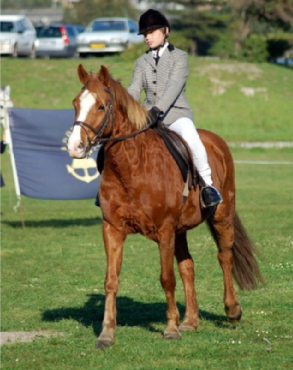
\includegraphics[width=\textwidth]{plots/segmentationImage.png}
		\caption{Original image}
        \end{subfigure}
	~
	\begin{subfigure}{0.27\textwidth}
                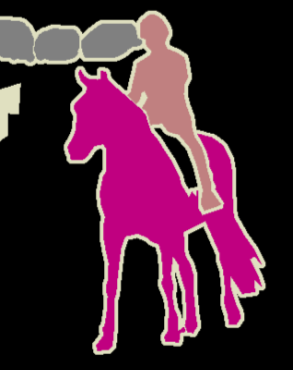
\includegraphics[width=\textwidth]{plots/segmentationTruth.png}
		\caption{Segmentation}
        \end{subfigure}
	\caption[Segmentation of an image]{Segmentation of an image with five classes. Image courtesy of~\cite{Long2015}}
	\label{fig:imageSegmentation}
\end{figure}
We segment an image by training a classifier on small patches, sliding it across bigger images to obtain per-pixel predictions and assigning each pixel to its highest predicted class.
%~\footnote{For classification, we average score vectors across pixels to obtain a single vector for the bigger image.}
Convolutional networks automatically behave this way when presented with an image bigger than those used for training, albeit, due to subsampling in the pooling layers, they produce a coarse segmentation that needs to be upsampled to match the size of the original image.
For instance, a convolutional network trained with $32\times 32$ images and two pooling layers (that reduce the input by a factor of 4) acts as a $32 \times 32$ filter with stride 4 in big images, so for a $256 \times 256$ image it will produce a $64 \times 64$ segmentation~\footnote{Padding the original image by $\lfloor (f_s-1)/2\rfloor = 15$ where $f_s = 32$ is the filter size} that needs to be upsampled by a factor of 4 to recover the original dimensions. 
\begin{comment}
We could also set a stride of 4 in the first (converted) fully connected layer to get score matrices of size $3\times 3$ for each 9 non-overlapping $32\times 32$ partitions of the original image. It works exactly as if we applied the convolutional network to the original image at a stride of 32 but does all computations in just one pass.
if we augment the stride of the firs fully connected layer we can compute coarser segmentations or
\end{comment}
Convolutional networks transform image segmentation into an end-to-end, learnable task.

%For training, the loss function sums the loss over all pixels; to account for the mismatch between the output of the network and the ground truth image (labels), which has the dimensions of the original image, we downsample the ground truth image or append an upsampling layer at the end of the network. This layer computes a differentiable function either fixed such as bilinear interpolation or learned such as a linear mapping; adding this upsampling layer forms a \emph{fully convolutional network}~\cite{Long2015}.
For training, the loss function sums the loss over all pixels; to account for the mismatch between the output of the network and the labelled image---the ground truth segmentation---, which has the dimensions of the original image, we downsample the labelled image or append an upsampling layer at the end of the network. This layer computes a differentiable function either fixed such as bilinear interpolation or learned such as a linear mapping; adding this upsampling layer forms a \emph{fully convolutional network}~\cite{Long2015}.

Evaluation metrics are the pixel-wise version of those used in classification (Sec.~\ref{sec:Classification}). For instance, accuracy is the proportion of correctly classified pixels averaged over all images.
%Another popular metric is the intersection over union (IOU) which can be calculated from the confusion matrix (Tab.~\ref{tab:ConfusionMatrix}) as TP/TP+FN+FP.

If we are interested in a particular class, e.g. object vs. background, we present a single score map showing its probability distribution across every position in the image. We can refine this map using gaussian smoothing, cluster-based thresholding, conditional random fields, among others. Finally, we threshold the post-processed map at some specific value to produce a segmentation; the threshold can be chosen using a validation set.
